% 5implementacja
\newpage

\section{Implementacja}

\paragraph{}
Przedstawioną metodę zaimplementowano w języku C++, przy użyciu elementów języka dodanych przy standaryzacji w wersji C++11/14. Wykorzystano również następujące biblioteki:
\begin{itemize}
	\item glm - (OpenGL Mathematics) biblioteka zawierająca funkcje i klasy wykorzystywane przy operacjach matematycznych. W zamyśle naśladuje zapis OpenGL Shading Language (GLSL).
	\item OpenGL - (ang. Open Graphics Library) API służące do tworzenia grafiki.
	\item GLEW - (OpenGL Extension Wrangler) biblioteka pomocna przy ładowaniu odpowiednich elementów biblioteki OpenGL.
	\item GLFW - biblioteka zawiera zestaw funkcji ułatwiających m.in. tworzenie okna dla aplikacji wykorzystujących OpenGL i obsługę urządzeń wejściowych (klawiatury, myszki, joysticka).
\end{itemize}
Kod źródłowy aplikacji dostępny jest w publicznym repozytorium kodu pod adresem:\\ \href{https://github.com/filu005/SPH}{https://github.com/filu005/SPH}.
\par


\begin{figure}
\subsection{Algorytm}
\subsubsection{Schemat blokowy aplikacji}

\centering
\caption{Diagram}
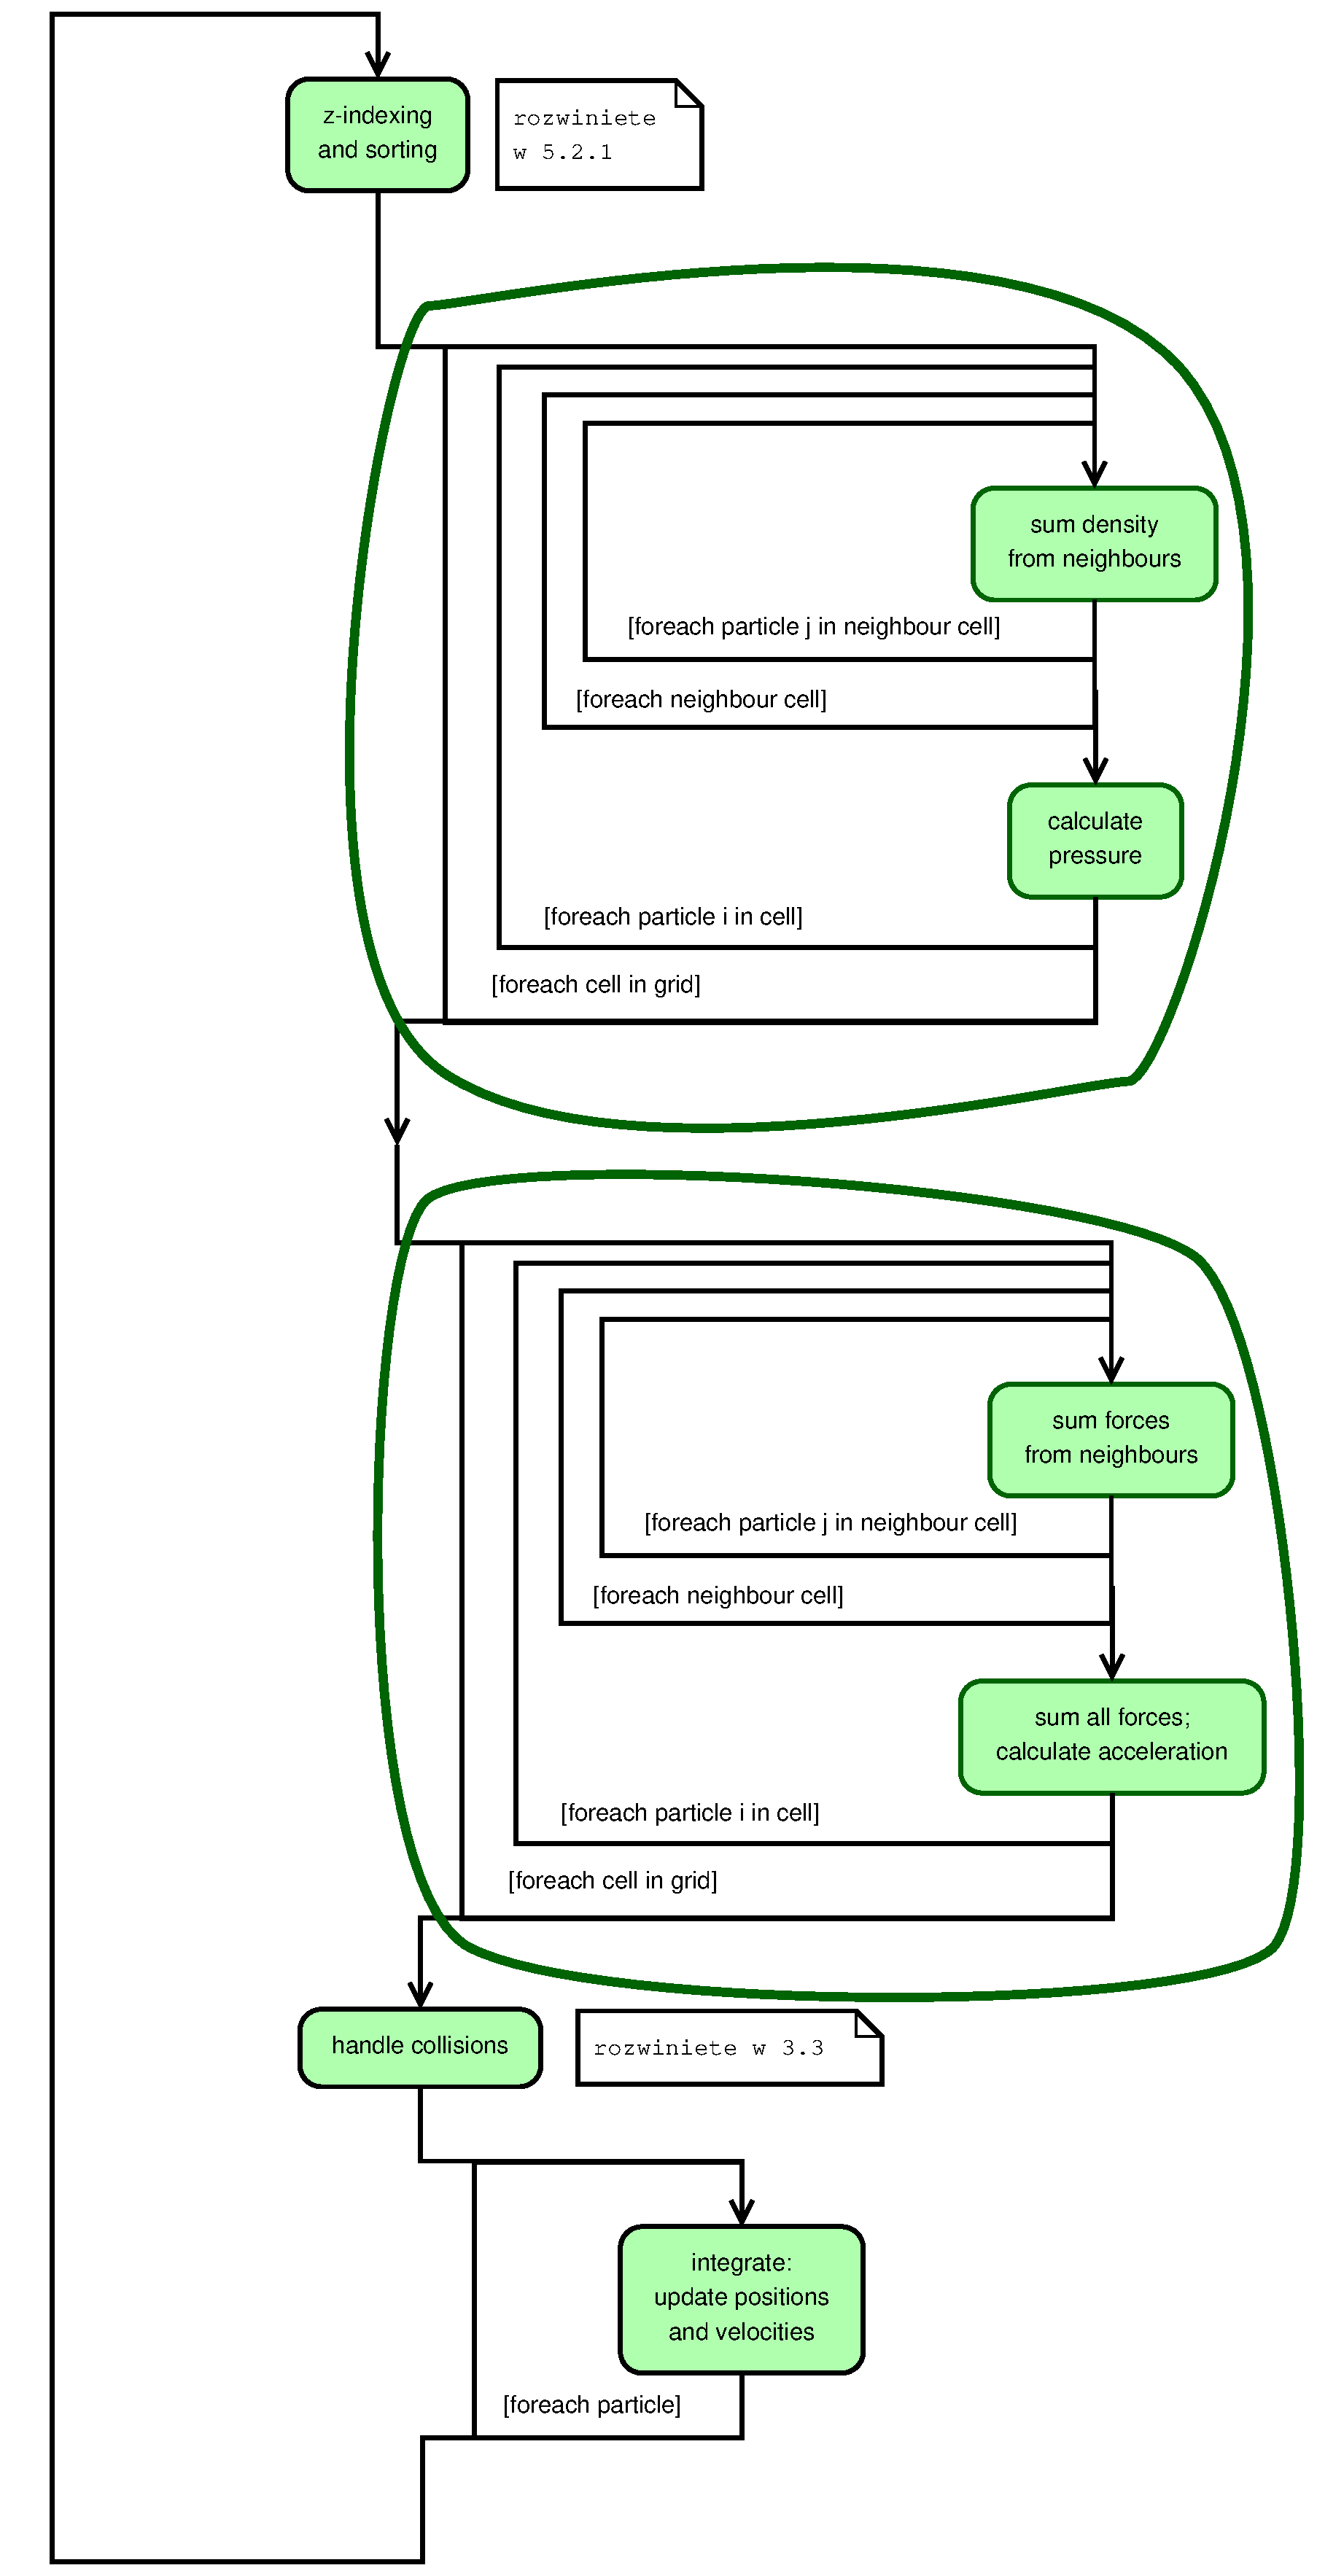
\includegraphics[width=350pt,keepaspectratio]{diagram.eps}%width=\textwidth,height=\textheight,
\label{fig:diagram_main}
\newpage
\end{figure}
\newpage

\subsubsection{Pseudokod algorytmu symulacji (?)}

\paragraph{}

\par

\subsubsection{Złożoność obliczeniowa (?)}

\paragraph{}

\par


\subsection{Optymalizacje}

\paragraph{}
Wydajność aplikacji poprawiać można na wiele sposobów. Najwięcej czasu pochłaniają obliczenia matematyczne związane z symulacją. Tutaj z pomocą przychodzą metody wyszukiwania sąsiadów cząstki koniecznych do obliczenia fizycznych właściwości. Kolejnym `wąskim gardłem' jest czas dostępu do pamięci RAM więc istotna jest lokalność danych i porządkowanie ich w pamięci podręcznej. Odrębnym tematem jest optymalizacja renderowania powierzchni płynu. <<zrównoleglanie obliczeń i GPGPU>>
\par

\subsubsection{Wyszukiwnie sąsiadów}
\label{subsubsec:neighbour_search}
<<uniform grid - jednorodna siatka>>
\paragraph{}
Obliczając parametr symulacji dla każdej cząsteczki przy użyciu SPH iteruje się po wszystkich pozostałych cząsteczkach. Jako, że dla każdej cząsteczki musimy poznać jej parametry, złożoność iteracyjna dla $n$ cząsteczek jest <<ograniczona przez>> $O(n^2)$. Chcąc symulować płyn opisany liczbą cząsteczek rzędu 10'000 w czasie rzeczywistym, taka złożoność obliczeniowa jest niesatysfakcjonująca. Aby <<zredukować>> złożoność obliczeniową stosuje się metody wyszukiwania sąsiadów.
\par
Wykorzystywane w symulacji jądra wygładzające posiadają tzw. promień odcięcia, który ogranicza zasięg jaki jest brany pod uwagę przy obliczaniu parametrów pojedynczej cząstki. Wiedząc, że cząstka wykorzystuje jedynie małą część innych cząstek do wyliczenia swoich parametrów, można znacznie skrócić czas obliczeń. W takim wypadku asymptotyczna złożoność obliczeniowa redukowana jest z $O(n^2)$ do $O(mn)$, gdzie $m$ oznacza średnią liczbę sąsiadów cząstki. Ta liczba często nie przekracza wartości 30-40.
\par

\paragraph{}
Jednym z typów struktur, które pozwalają poszeregować cząsteczki na grupy sąsiadów jest jednorodna siatka (ang. uniform grid). Cały obszar, w którym znajdują się cząsteczki - i mogą się znaleźć podczas przebiegu symulacji - dzielony jest na komórki. Obszar ten nie zmienia się przez cały czas trwania symulacji więc istotne jest aby cząsteczki nie miały szansy z niego `uciec'. W przeciwnym wypadku algorytm nie będzie w stanie poprawnie znaleźć sąsiadów dla `uciekinierów'. Przy obliczaniu parametrów cząsteczek znajdujących się w komórce $X$ iteruje się tylko po tych cząsteczkach, które znajdują się w 26 komórkach <<ref: (tj. w promieniu jednej komórki; za wyjątkiem komórek znajdujących się na skraju obszaru)>> sąsiadujących z komórką $X$. Rozmiar komórek również jest stały i jest równy najbliższej potędze dwójki większej od promienia odcięcia jądra wygładzającego. Przyjęcie takiego rozmiaru komórki zapewnia, że sąsiadujące komórki zawierają wszystkie cząsteczki wymagane do przeprowadzenia poprawnych obliczeń.
\par
Każdej komórce może zostać przypisany indeks, który oblicza się \textbf{dla cząsteczki} według poniższego wzoru, na podstawie jej położenia:

\begin{equation}
c_{idx} = k + l * K + m * K * L
\label{eqn:get_cell_index}
\end{equation}
gdzie $K$ i $L$ to rozmiary obszaru symulacji w kierunkach $x$ i $y$ <<uwaga, że K i L to potęgi dwójki aby nie wprowadzać niedokładności związanych z zaokrągleniami przy dzieleniu>>, a $[k, l, m]$ to położenie komórki w globalnym układzie współrzędnych. <<Implementacja funkcji w dodatku/listingu xxx>>.

\paragraph{}
Aby zachować optymalne ułożenie danych w pamięci podręcznej, tablica przechowująca cząsteczki jest sortowana ze względu na indeks komórek w której znajdują się cząsteczki - czyli pośrednio ze względu na ich położenie w obszarze symulacji. Dzięki temu cząsteczki znajdujące się w jednej komórce ułożone są blisko siebie również w pamięci. Nie oznacza to jednak, że cząsteczki z sąsiadujących komórek - które również biorą udział w obliczeniach - będą znajdywały się również niedaleko w pamięci. Aby zwiększyć wykorzystanie danych znajdujących się w pamięci podręcznej (ang. cache-hit) wykorzystywana jest Krzywa Hilberta/Krzywa-Z (ang. Hilbert space filling curve/Z-Curve) <<ref Hilbert curve>>. Indeksowanie komórek i sortowanie cząsteczek według tej krzywej pozwala na ułożenie cząsteczek znajdujących się w sąsiadujących komórkach bliżej siebie w pamięci. <<pomiary, grafika z z-curve>>
\par
Posortowanie cząsteczek pozwala również na uproszczenie struktury komórki, która przy takich założeniach przechowuje jedynie \textbf{adres pierwszej cząsteczki} w posortowanej tablicy i \textbf{liczbę cząsteczek} znajdujących się w danej komórce. <<graficzna reprezentacja siatki, listing xxx>>
%układ, rozkład, schemat, podział, organizacja, powiązanie, ulozenie
\par

\paragraph{}
Cały opisany powyżej proces optymalizacji wyszukiwania sąsiadów przedstawiony jest na poniższym schemacie:
\par
%schemat blokowy `z-index sort search'
\begin{figure}[h]
\centering
\caption{Diagram indeksowania i szeregowania cząsteczek}
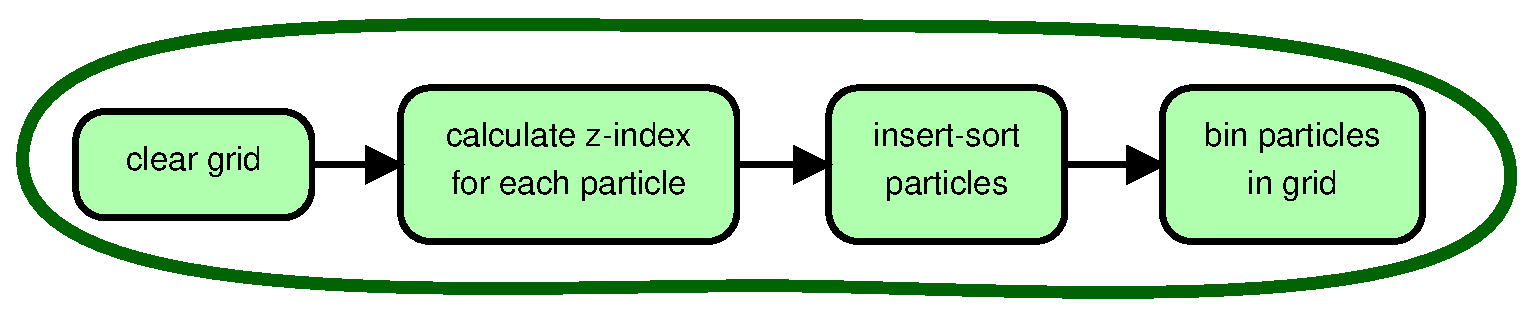
\includegraphics[width=450pt,keepaspectratio]{diagram_zindex.eps}
\label{fig:diagram_zindex}
\end{figure}

\subsection{Całkowanie numeryczne}

\paragraph{}

\par

\subsubsection{Krok czasowy}

\paragraph{}

\par

\subsection{Parametry symulacji}

\paragraph{}
Płyn symulowany metodą SPH można <<formułować>> nadając wartości kilku stałych opisujących ten płyn. Niektórych wartości parametrów nie można jednak przepisać bezpośrednio z tablic stałych fizycznych, ponieważ w <<obszarze>> na jakim przeprowadzana jest symulaja nie mają takiego sensu jak w rzeczywistym świecie i nie <<powodują/inicjują>> spodziewanych efektów. Ich wielkości muszą być także dostrajane z myślą o stabilności symulacji, na którą mają duży wpływ. Powyższe kwestie sprawiają, że ustawianie stałych płynu - przynajmniej na początkowych etapach implementacji symulatora - jest trudne i odbywa się metodą prób i błędów. Poniżej umieszczone zostały przykładowe wartości tych parametrów, które dobrze sprawdzają się dla symulacji płynów skonstruowanym algorytmem oraz wskazówki jak dobierać te wielkości.
\par

\subsubsection{Objętość symulowanego płynu oraz masa pojedynczej cząsteczki}

\paragraph{}
Masa pojedynczej cząsteczki wpływa na wielkość sił powstających przy symulacji. Ten parametr jest <<dosyć>> czuły i istotnie wpływa na charakterystykę symulacji jak i jej stabilność. Jego dopasowanie powinno przebiegać równolegle z korektą przede wszystkim kroku czasowego oraz promienia odięcia jądra wygładzającego.
\par

\subsubsection{Promień odcięcia jądra wygładzającego}

\paragraph{}
Promień odcięcia $h$ wyrażany w $[m]$ jest wartością mającą duży wpływ na stabilność i wydajność symulacji oraz jakość odwzorowania płynu. Określa on <<`zasięg widzenia'>> pojednczej cząsteczki, w którym to szuka swoich sąsiadów - cząsteczek wykorzystywanych do obliczeń parametrów tej cząsteczki. Im więcej sąsiadów, tym zoptymalizowany algorytm ich przeszukiwania \eqref{subsubsec:neighbour_search} osiąga gorszą złóżoność, która z powrotem dąży do $O(n^2)$. Mylnym jest pojęcie o zwiększaniu dokładności symulacji wraz ze zwiększeniem promienia odcięcia. Od pewnego momentu zwiększanie tego parametru powoduje nienaturalne zachowanie się płynu. Siła ciśnienia, która jest odpowiedzialna za utrzymywanie odpowiednich odlegości pomiędzy cząsteczkami staje się zbyt duża i cząsteczki zlepiaja się w kulę lub torusa <<foto>>.
\par Promień odcięcia może być również zbyt mały. W takim wypadku zbyt mała liczba cząstek jest brana pod uwagę przy obliczaniu parametrów i symulacja znowu staje się nienaturalna. Dodatkowo mały promień negatywnie wpływa na stabilność symulacji.
\par
\paragraph{}
Ustawianie tego parametru, spowodowane przez jego duży wpływ na charakter symulacji, jest trudne. Często sprowadza się do wielokrotnego testowania ustawień tego parametru w parze z innymi, mającymi wpływ na stabilność i wizualną jakość symulacji. W tej implementacji zdecydowano się na dopasowanie promienia odcięcia do wielkości oczka siatki przechowującej sąsiadów cząstki (patrz rozdział \eqref{subsubsec:neighbour_search}) tak aby te dwie wielkości były jak najbardziej zbliżone. Zostało zbadane, że taki stosunek tych wielkości jest optymalny ze względu na wydajność przeszukiwania sąsiadów <<ref eurographics freiburg 2014>>.
\par

\subsubsection{Gęstość spoczynkowa}

\paragraph{}
Równanie \eqref{eqn:sph_desbrun_pressure} wykorzystuje gęstość spoczynkową do obliczenia ciśnienia dla pojedynczej cząsteczki. Mała wartość tego parametru powoduje, że siła ciśnienia pomiędzy cząsteczkami wzajemnie je odpycha. Odpowiednio go korygując powodujemy zmniejszenie się tej siły odpychającej. W pewnym momencie siła osiąga wartości ujemne i cząsteczki zaczynają się przyciągać. Zbyt duża wartość prowadzi do szybkiego wzrostu wartości ciśnienia co powoduje eksplozję numeryczną.
\par

\subsubsection{Lepkość}

\paragraph{}
Stała występująca w równaniu \eqref{eqn:sph_force_viscosity} na siłę lepkości dostosowywana jest ze względu na pożądany charakter symulowanego płynu oraz efekt `wygładzający', który zapobiega nagłym wzrostom prędkości cząsteczek i stabilizuje symulację.
\par

\subsubsection{Napięcie powierzchniowe}

\paragraph{}
W równaniu \eqref{eqn:sph_force_surface_tension} występuje stała $\sigma$ modulująca siłę przyciągania do siebie cząstek znajdujących się na powierzchni płynu. Jej większa wartość powoduje zwiększenie się tej siły.
Wartość progu $l$ funkcjonującego w równaniu \eqref{eqn:sph_force_surface_tension_threshold} ma jedynie ustrzec przed dzieleniem przez bardzo małe wartości. Wartość progu powinna być niska aby zachować naturalność działania siły napięcia powierzchniowego.
\par